% =====================================================================
\section{Overall forecast performance}\label{sec:overall}

\subsection{Validation and held-out test results}
\Cref{tab:results} reports validation medians, which guided model selection, alongside the final test metrics, which are the evidence for our conclusions. Validation and test give the same ranking of methods. Errors are uniformly larger on the test drifters, by 3.1--10.5\% in median (CV \SI{15.04}{km} on validation against \SI{15.89}{km} on test, +5.6\%; \GBH{} \SI{8.51}{km} against \SI{9.23}{km}, +8.5\%). The untuned CV baseline shifts as well, so part of the difference reflects the composition of the two sets of 78 drifters; the test drifters are, for example, faster on average (\cref{sec:motion}). However, the History variants shift more in relative terms (8.2--10.5\%) than CV, and validation estimates of models chosen as the best of several configurations are expected to be optimistic. Some validation-set optimism from hyperparameter selection therefore cannot be ruled out. For this reason, all conclusions rest on the test results, on which no choice was made.

\begin{table}[!htbp]
\centering
\caption{Validation median and held-out test error (km) for all methods on identical cases. The last column is the reduction in test median relative to Constant Velocity (negative means worse). Test set: \num{82546} forecasts from 78 drifters. Best values in bold.}
\label{tab:results}
\small
\begin{tabular}{@{}lrrrrrr@{}}
\toprule
 & Validation & \multicolumn{4}{c}{Test} & Median vs CV \\
\cmidrule(lr){2-2}\cmidrule(lr){3-6}
Method & median & mean & median & P90 & RMSE & (\%) \\
\midrule
Constant Velocity    & 15.04 & 20.55 & 15.89 & 40.90 & 26.77 & -- \\
Mean-flow Advection  & 22.37 & 32.38 & 24.28 & 68.80 & 42.05 & $-52.8$ \\
\addlinespace
Ridge Current        & 13.24 & 18.49 & 14.14 & 37.70 & 24.00 & 11.0 \\
Ridge History        & 10.48 & 16.15 & 11.58 & 33.56 & 22.20 & 27.1 \\
Elastic Net Current  & 13.11 & 18.29 & 13.95 & 36.94 & 23.90 & 12.2 \\
Elastic Net History  & 10.49 & 16.16 & 11.60 & 33.59 & 22.23 & 27.0 \\
\addlinespace
RF Current           & 12.62 & 17.00 & 13.05 & 34.37 & 22.07 & 17.8 \\
RF History           &  8.54 & 13.33 &  9.25 & 28.81 & 18.78 & 41.7 \\
ET Current           & 12.61 & 17.12 & 13.16 & 34.65 & 22.20 & 17.2 \\
ET History           &  8.63 & 13.37 &  9.33 & 28.91 & \textbf{18.75} & 41.2 \\
GB Current           & 12.66 & 16.89 & 13.05 & 34.05 & 21.83 & 17.9 \\
GB History           & \textbf{8.51} & \textbf{13.23} & \textbf{9.23} & \textbf{28.55} & 18.60 & \textbf{41.9} \\
\bottomrule
\end{tabular}
\end{table}

\begin{figure}[!htbp]
  \centering
  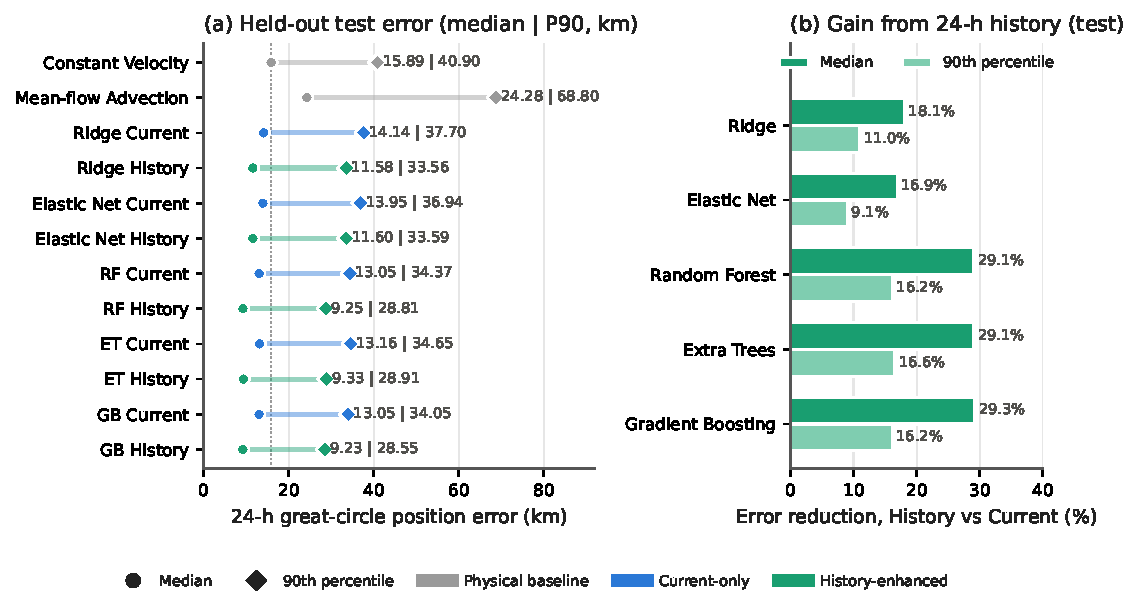
\includegraphics[width=\textwidth]{figures/generated/fig_test_model_comparison.pdf}
  \caption{Held-out test performance. (a) Median (circle) and P90 (diamond) error for all twelve methods; the dotted line marks the CV median. (b) Relative reduction in median and P90 error from adding history features within each model family. Generated from \texttt{models/final\_test\_comparison.csv}; no model was re-evaluated.}
  \label{fig:test}
\end{figure}

\paragraph{Sensitivity to tuning.} Validation results were insensitive to the Ridge penalty (medians within \SI{0.02}{km} across $\alpha$ for both variants) and, for the Current tree models, to tree complexity (RF, ET and GB Current medians within \SIrange{12.61}{12.71}{km} across configurations). The History tree models, by contrast, improved steadily with capacity: GB History from \SI{9.11}{} to \SI{8.51}{km}, RF History from \SI{8.83}{} to \SI{8.54}{km} and ET History from \SI{9.30}{} to \SI{8.63}{km} across their three configurations. History information is therefore what gives the extra model capacity something to learn, and the History models might improve further beyond the grids tested.

\paragraph{Learned corrections outperform both physical baselines.} Every learned model improves on Constant Velocity in all four metrics. \GBH{} reduces the test median by 41.9\% (\SI{15.89}{}$\to$\SI{9.23}{km}), the mean by 35.6\%, P90 by 30.2\% and RMSE by 30.5\% (\cref{fig:test}a). A 24-hour displacement correction learned from the drifters' own kinematics therefore removes a substantial part of the error made by assuming that velocity persists.

\paragraph{The empirical mean flow is a weak baseline.} Mean-flow Advection is the least accurate method (median \SI{24.28}{km}, P90 \SI{68.80}{km}), roughly 50\% worse than Constant Velocity. A stationary, seasonally averaged field on a \ang{1} grid smooths away the meanders and eddies that dominate a particular drifter's next 24 hours. Averaging across a narrow jet is also likely to dilute peak speeds, although we did not quantify this. The current velocity, by contrast, already contains this synoptic information. \Cref{sec:motion} shows that the mean flow is nonetheless competitive in one specific regime.

\paragraph{History features matter more than model flexibility.} Within every family, the History variant beats its Current counterpart (\cref{fig:test}b). The median reduction is 18.1\% for Ridge, 16.9\% for Elastic Net, and 29.1--29.3\% for Random Forest, Extra Trees and Gradient Boosting. Flexibility alone helps less: among Current models, moving from Ridge to Gradient Boosting lowers the median by only \SI{1.09}{km} (\SI{14.14}{}$\to$\SI{13.05}{km}), whereas adding history to Gradient Boosting lowers it by \SI{3.82}{km}. The two effects interact. In relative terms, history helps the tree ensembles roughly 1.6--1.7 times as much as it helps the linear models, which suggests that the useful information in the history summaries enters partly through nonlinear combinations, for example a velocity trend whose implication depends on current speed. For Gradient Boosting, the overall mean paired reduction from history is \SI{3.65}{km} with a 95\% drifter-cluster bootstrap interval of \SIrange{3.14}{4.14}{km} (\cref{sec:bootstrap}). The benefit is therefore not an artefact of a few long tracks. It is also not universal: in a report-time check of the saved predictions, \GBH{} beat \GBC{} in 71.4\% of individual test forecasts.

\paragraph{Typical errors improve more than tail errors.} The relative gain in P90 is consistently smaller than in the median: 16.2\% against 29.3\% for history within Gradient Boosting, and 30.2\% against 41.9\% for \GBH{} against CV. Even the best model's P90 (\SI{28.5}{km}) is three times its median, so roughly one forecast in ten remains in error by more than \SI{28}{km}. For applications driven by worst cases, the residual tail is as important as the improvement in the centre.

\paragraph{The three tree ensembles are practically equivalent.} RF, ET and GB History differ by at most \SI{0.10}{km} in test median and \SI{0.36}{km} in P90, and these differences have not been assessed against drifter-level sampling variability. We therefore do not rank them. Gradient Boosting is preferred on practical grounds: on the same machine, the selected configuration trained in about \SI{6}{s}, compared with about \SI{41}{s} for Extra Trees and \SI{173}{s} for Random Forest (validation runs, notebook cells 31--34), and its saved model is roughly 2\,MB, compared with hundreds of megabytes for the bagged ensembles.

\subsection{Trajectory-level behaviour}\label{sec:trajectories}
\Cref{fig:traj} joins successive rolling 24-hour forecast endpoints for the three test drifters with the most test forecasts, over the first seven days of each drifter's longest continuous segment. The drifters were chosen by data coverage, not accuracy, but three drifters are illustrations, not a representative sample.

\begin{figure}[!htbp]
  \centering
  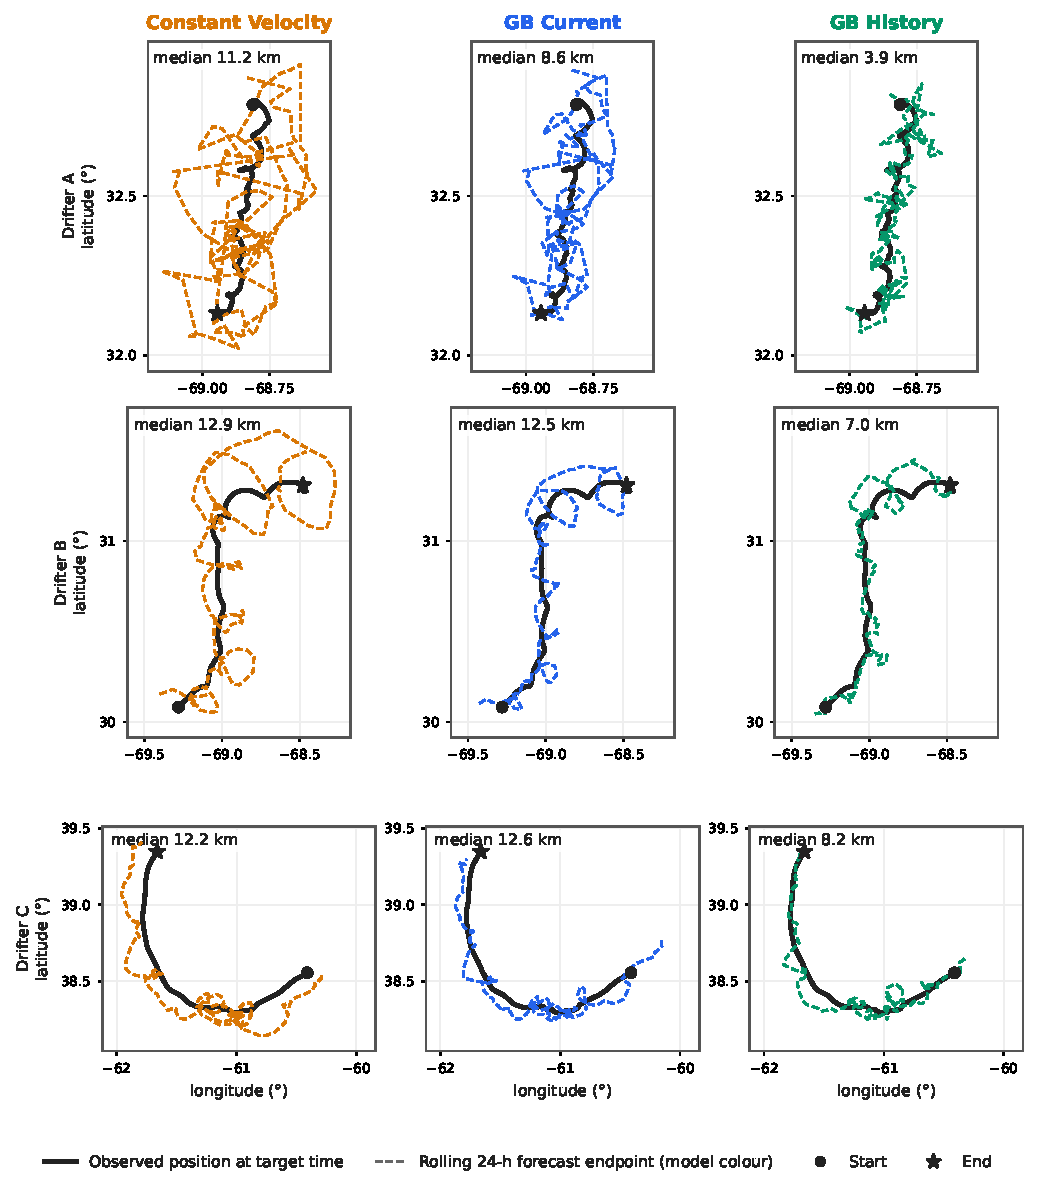
\includegraphics[width=0.86\textwidth]{figures/generated/fig_traj_cv_gb.pdf}
  \caption{Observed positions at target times (black) and rolling 24-hour forecast endpoints (dashed) for CV, \GBC{} and \GBH{}, for three held-out drifters (A: 139080, B: 300234063940890, C: 300234064909860) over seven days (circle: start; star: end). Each dashed vertex is an independent forecast issued 24\,h earlier from the observed state, not a simulated trajectory. In-panel values are window-specific median errors. Axes are fixed per drifter across this figure and \cref{fig:family,fig:family2}. Re-plotted for legibility from saved test predictions with the selection rules of notebook cell 44, reproducing its panel medians.}
  \label{fig:traj}
\end{figure}

Three patterns recur. First, CV endpoints scatter widely and form loops around the observed path. This pattern is consistent with short-period fluctuations in the instantaneous velocity being extrapolated over a full day, although we did not test that mechanism. Second, \GBC{} contracts the scatter but keeps much of its structure, since it sees only the same instantaneous state. Third, \GBH{} follows the observed path most closely, including through the bend of the third drifter (window medians \SI{3.9}{}, \SI{7.0}{} and \SI{8.2}{km}, against \SI{11.2}{}, \SI{12.9}{} and \SI{12.2}{km} for CV). It still shows local jitter between consecutive forecasts: accurate endpoints do not imply a smooth sequence of forecasts. The family comparisons in \cref{fig:family,fig:family2} (\cref{app:figs}) show the same picture: Ridge and Elastic Net produce nearly identical tracks, and RF, ET and GB History are visually indistinguishable, matching \cref{tab:results}.

\Cref{fig:cases} shows four single forecasts chosen by reproducible rules. The two history-related cases come from the same drifter, which illustrates that the benefit of history varies along one trajectory. In the ``difficult'' case (the 95th percentile of \GBH{} error), every model extrapolates roughly along the recent north-eastward direction of travel and misses the subsequent curve in the observed path. In the ``history helps'' case, \GBH{} reduces the error relative to \GBC{} but still misses by \SI{55.5}{km}: the drifter travels much farther west-southwest than any model predicts. In the ``history hurts'' case, the history model over-extrapolates northward while \GBC{} lands closer. These examples make concrete why the error distribution has a heavy upper tail: some 24-hour futures are simply not predictable from the preceding day of kinematics.

\begin{figure}[!htbp]
  \centering
  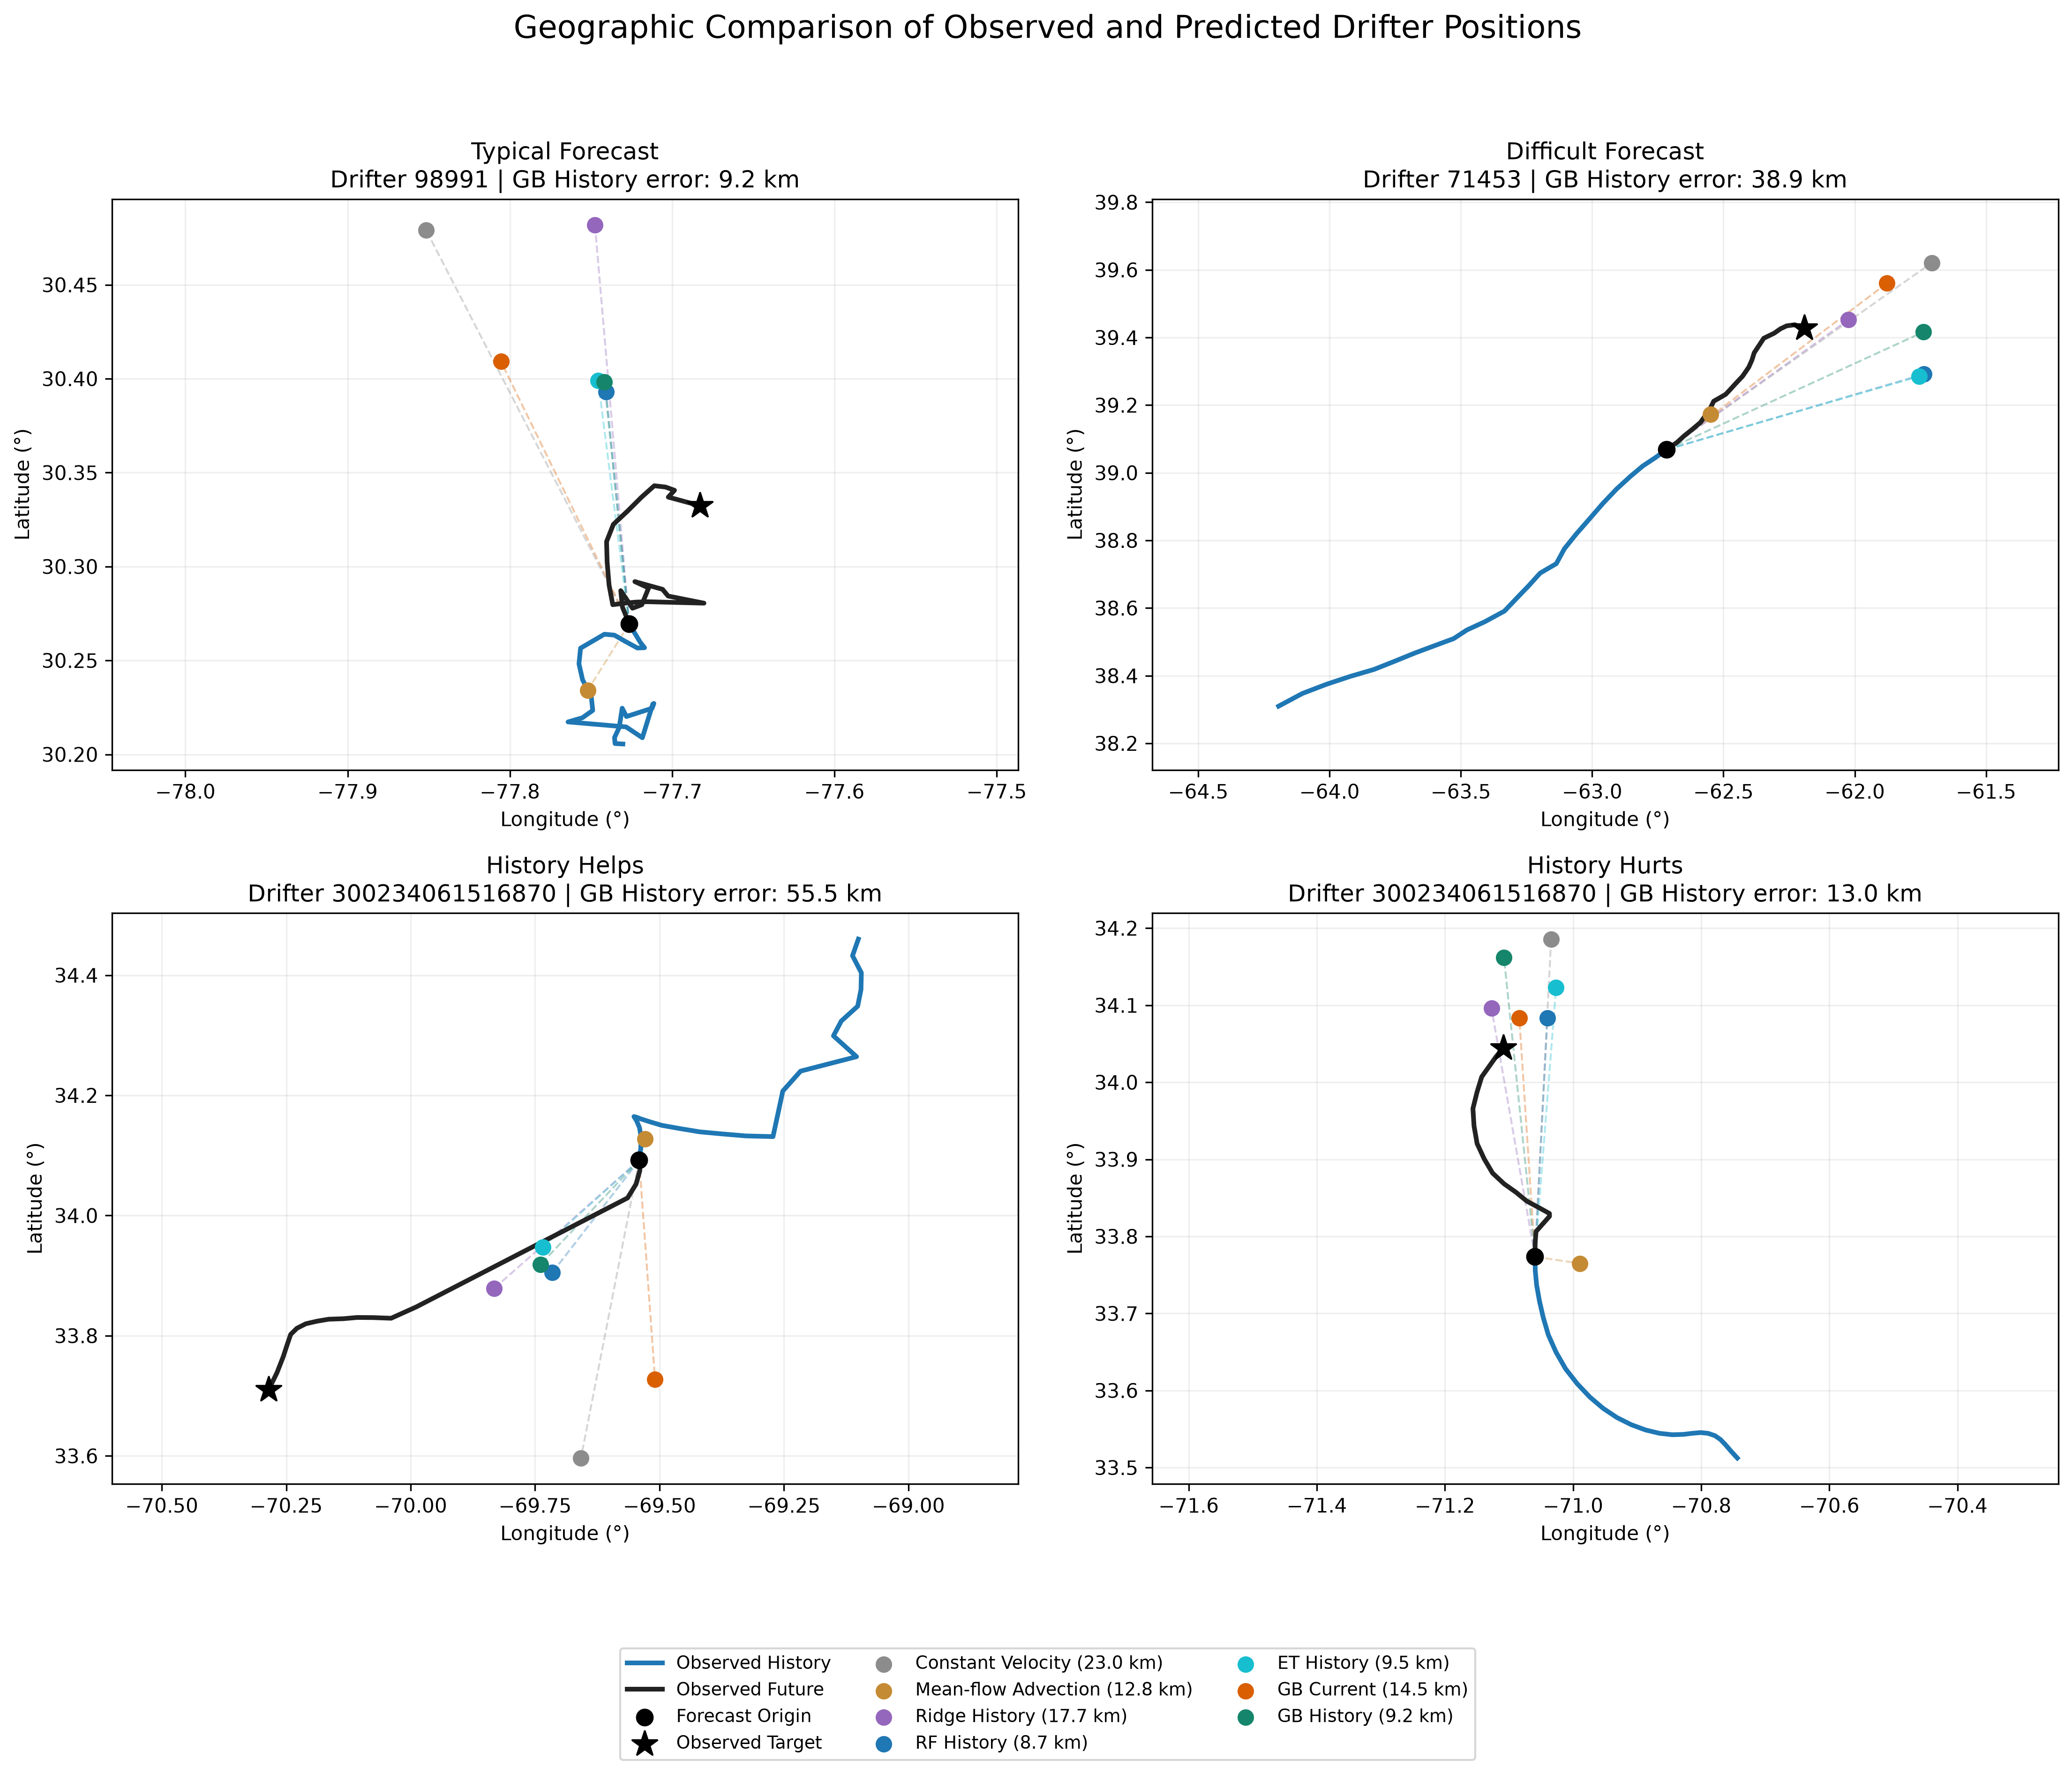
\includegraphics[width=\textwidth]{figures/report_geographic_forecast_cases.png}
  \caption{Single-forecast case studies on test drifters: typical (\GBH{} error closest to its median), difficult (closest to its 95th percentile), and history helps or hurts (5th and 95th percentiles of the paired gain $E^{\mathrm{GBC}}-E^{\mathrm{GBH}}$). Blue: observed 24-h history; black: observed future; dots: predicted endpoints. \emph{The error values in the shared legend refer to the ``Typical'' panel only}; panel titles give \GBH{} errors. Source: notebook cell 41.}
  \label{fig:cases}
\end{figure}
